%! Author = J. Villing
%! Date = 24.07.21

% Preamble
\documentclass[final]{fhnwreport}
% Packages
\usepackage{amsmath}
\usepackage{lipsum}
\usepackage[german]{babel}
\usepackage[style=ieee,urldate=comp,backend=biber]{biblatex}
\usepackage{listings}
\usepackage{pdflscape}
\usepackage{xcolor}
\usepackage{dirtree}
\usepackage{textcomp}
\usepackage{tabularx}
\usepackage{blindtext}
\usepackage{import}
\usepackage{float}
\addbibresource{main.bib}
\graphicspath{{./images/}}

% Custom JS Listing support
\definecolor{mygreen}{rgb}{0,0.6,0}
\definecolor{mygray}{rgb}{0.5,0.5,0.5}
\definecolor{mymauve}{rgb}{0.58,0,0.82}
%Customize a bit the look
\lstset{ %
    backgroundcolor=\color{white}, % choose the background color; you must add \usepackage{color} or \usepackage{xcolor}
    basicstyle=\footnotesize, % the size of the fonts that are used for the code
    breakatwhitespace=false, % sets if automatic breaks should only happen at whitespace
    breaklines=true, % sets automatic line breaking
    captionpos=b, % sets the caption-position to bottom
    commentstyle=\color{mygreen}, % comment style
    deletekeywords={...}, % if you want to delete keywords from the given language
    escapeinside={\%*}{*)}, % if you want to add LaTeX within your code
    extendedchars=true, % lets you use non-ASCII characters; for 8-bits encodings only, does not work with UTF-8
    frame=single, % adds a frame around the code
    keepspaces=true, % keeps spaces in text, useful for keeping indentation of code (possibly needs columns=flexible)
    keywordstyle=\color{blue}, % keyword style
% language=Octave, % the language of the code
    morekeywords={*,...}, % if you want to add more keywords to the set
    numbers=left, % where to put the line-numbers; possible values are (none, left, right)
    numbersep=5pt, % how far the line-numbers are from the code
    numberstyle=\tiny\color{mygray}, % the style that is used for the line-numbers
    rulecolor=\color{black}, % if not set, the frame-color may be changed on line-breaks within not-black text (e.g. comments (green here))
    showspaces=false, % show spaces everywhere adding particular underscores; it overrides 'showstringspaces'
    showstringspaces=false, % underline spaces within strings only
    showtabs=false, % show tabs within strings adding particular underscores
    stepnumber=1, % the step between two line-numbers. If it's 1, each line will be numbered
    stringstyle=\color{mymauve}, % string literal style
    tabsize=2, % sets default tabsize to 2 spaces
    title=\lstname % show the filename of files included with \lstinputlisting; also try caption instead of title
}
%END of listing package%

\definecolor{darkgray}{rgb}{.4,.4,.4}
\definecolor{purple}{rgb}{0.65, 0.12, 0.82}

%define Javascript language
\lstdefinelanguage{JavaScript}{
    keywords={typeof, new, true, false, catch, function, return, null, catch, switch, const, let, var, if, in, while, do, else, case, break},
    keywordstyle=\color{blue}\bfseries,
    ndkeywords={class, export, boolean, throw, implements, import, this},
    ndkeywordstyle=\color{darkgray}\bfseries,
    identifierstyle=\color{black},
    sensitive=false,
    comment=[l]{//},
    morecomment=[s]{/*}{*/},
    commentstyle=\color{purple}\ttfamily,
    stringstyle=\color{red}\ttfamily,
    morestring=[b]',
    morestring=[b]"
}

\lstset{
    language=JavaScript,
    extendedchars=true,
    basicstyle=\footnotesize\ttfamily,
    showstringspaces=false,
    showspaces=false,
    numbers=left,
    numberstyle=\footnotesize,
    numbersep=9pt,
    tabsize=2,
    breaklines=true,
    showtabs=false,
    captionpos=b
}



\title{Google Docs Light}  %Project Title
\author{Workshop Web - FS22}                      %Document Type => Technical Report, ...

\begin{document}
    \maketitle

    \vspace*{\fill}

    \begin{center}
        \renewcommand\arraystretch{2}
        \begin{tabular}{l l}
            Studenten & P. Schmucki, J. Villing, K. Zellweger\\
            Dozenten & D. König, S. Meichtry, J. Luthiger \\
            Studiengang & Informatik\\
            Hochschule & Hochschule für Technik
        \end{tabular}
    \end{center}

    \clearpage

%%---TABLE OF CONTENTS-------------------------------------------------------------------
    \setcounter{tocdepth}{2}
    \tableofcontents
    \clearpage

%%---TEXT--------------------------------------------------------------------------------
    \pagenumbering{arabic}
    \section{Ausgangslage}

Im Rahmen WOWEB.

Aufgabe: Google Docs Light.

Eine zentrale Anforderung an das System ist die konsistente und verzögerungsfreie Darstellung eines Dokuments auf mehreren Klienten.

Die Wahl eines geeigneten Kommunikationsprotokolls ist die Grundlage für eine erfolgreiche Lösung.

Archi und Impl Doku folgt.

    \section{Technologie Stack}

Eine zentrale Anforderung an das System ist die konsistente und verzögerungsfreie Darstellung eines Dokuments auf mehreren Klienten.
Die Wahl eines geeigneten Kommunikationsprotokolls ist die Grundlage für eine erfolgreiche Lösung.

Wir verwenden HTTP-Event Streams als Grundlage für die Kommunikation zwischen dem Backend Server und den Klienten.
Als konkrete Implementation dieser Technologie setzen wir Spring-WebFlux ein.
Die weitere Technologieauswahl orientiert sich an diesem Grundsatz Entscheid.

\subsection{Backend Server}
Spring WebFlux ist integriert in das Spring Boot Ökosystem und benötigt daher eine zugrundeliegende JVM\@.
Sprachen die auf der JVM aufbauen, haben den Vorteil, dass sie System Interoperabel sind.

Anstatt Java setzen wir jedoch auf Kotlin als Backend Sprache.
Bis jetzt hat kein Mitglied des Projektteams nennenswerte Erfahrung mit Kotlin und wir möchten diese Gelegenheit nutzen,
die Sprache in einem Projekt näher kennenzulernen.
Wir erwarten die nachfolgenden Vorteile: 

\begin{itemize}
    \item Robuste Implementierung dank Null Safety
    \item Weniger Boilerplate und damit übersichtlichere Implementeirung
    \item Effiziente und Übersichtliche Anwendung von Streams
    \item Schlanke Entitäten und Domänenklassen durch Data Classes
\end{itemize}


\subsection{Frontend Clients}
Kein Teammitglied hat bis jetzt vertiefte Erfahrung im Bereich der Frontend-Entwicklung.
Daher setzen wir auf das an der FHNW vermittelte Framework React, um die Clients zu implementieren.
React bietet mit seinem Komponenten-Model eine einfache Abstraktionsmöglichkeit um die Anwendung sauber zu Kapseln.
Die Funktionalen JSX Komponenten scheinen leichtgewichtiger im Vergleich zu den HTML-Template-Ansätzen von Angular oder VueJS\@.

Unser Ziel ist es in diesem Projekt die Kenntnisse in einem Projekt zu vertiefen und die Client-Software möglichst pur funktional zu halten.


\subsection{Datenbank System}
Um die kollaborativ erstellten Dokumente zu persistieren und zu verwalten setzen wir auf eine No-SQL Lösung.
Das notwendige Datenmodel lässt sich elegant als \emph{Document} abbilden.
Durch den Einsatz einer No-SQL Lösung kann die Representation der Dokumente über alle Layer der Applikation gleichbleibend beibehalten werden,
ohne die Notwendigkeit von ORM\@.

Konkret wird im Projekt MongoDB als Datenbanksystem verwendet.
Wir haben uns für diese Variante aufgrund der bestehenden reaktiven Integration in das Springframework entschieden.


\begin{figure}
    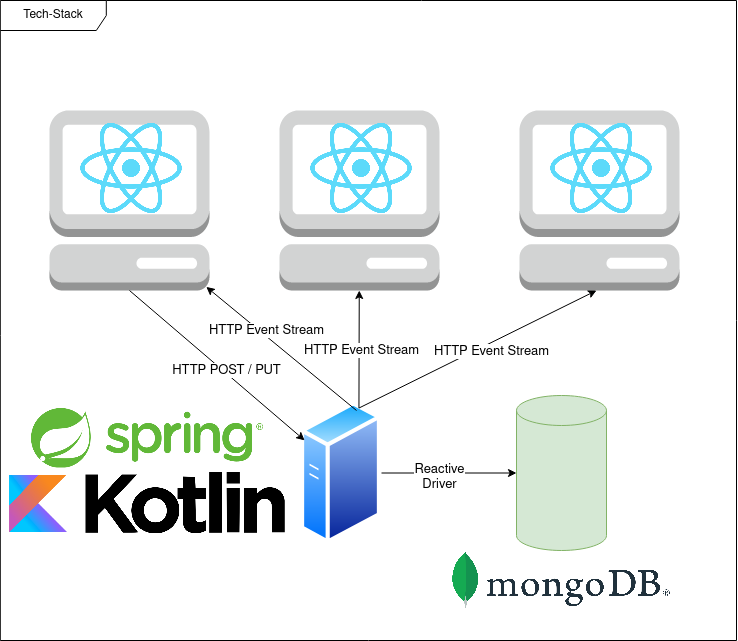
\includegraphics[width=\textwidth,height=\textheight,keepaspectratio]{TechStack}
    \caption{Technologie Stack}
\end{figure}

    \section{Systemübersicht}

\subsection{Lösungsstrategie}
Um die verteilte Dokumentenbearbeitung zu ermöglichen, verwenden wir eine Variante von Eventsourcing.
Dabei sollen die alle Änderungen am Dokument als einzelne Commands modelliert werden.
Commands werden von Clients generiert, lokal angewendet und anschliessend an den Server gesendet.
Dieser führt den Zustand des Dokuments und wendet Änderungen darauf an.
Allfällige Konflikte werden dabei auf dem Server gelöst.
Nach der Verarbeitung eines Commands veröffentlicht der Server alle angewendeten Commands sowie Commands zur Konfliktlösung.
Diese Commands werden wiederum von den Clients angewendet, um einen konsistenten Zustand des Dokuments herzustellen.
Commands werden in einer Datenbank persistiert.

Dieser Ansatz erlaubt es Änderungen nachzuvollziehen und bei Bedarf einen früheren Zustand des Dokuments wiederherzustellen.
Das Führen des Zustands auf dem Server erlaubt es, eine ''Source Of Truth'' zu haben, die den gültigen Zustand des Dokuments diktiert.
Das Anwenden von Commands in den Clients erlaubt es auch dort einzelne Änderungen nachzuvollziehen und darzustellen.

\subsection{Technologien und Systemaufbau}

Das Versenden von Commands findet über zwei getrennte Kanäle statt.
Für Versenden von Commands vom Backend an Clients verwenden wir HTTP-Event Streams (Server Sent Events).
Als konkrete Implementation dieser Technologie setzen wir Spring-WebFlux ein.
Die weitere Technologieauswahl orientiert sich an diesem Grundsatz Entscheid.
Für das Versenden von Commands von Clients an das Backend werden HTTP-POST-Requests verwendet.
Diese Trennung erlaubt es, das Schreiben und Lesen von Änderungen zu trennen.

\subsubsection{Backend Server}

Für das Backend wird eine Spring Boot Applikation mit Spring Webflux erstellt.
Dieser Ansatz ermöglicht es, eine reaktive Serverapplikation zu erstellen, welche mit minimalem Boilerplate Code auskommt.

Das Spring Boot Ökosystem benötigt eine zugrundeliegende JVM\@.
Sprachen die auf der JVM aufbauen, haben den Vorteil, dass sie System Interoperabel sind.
Anstatt Java setzen wir jedoch auf Kotlin als Backend Sprache.
Bis jetzt hat kein Mitglied des Projektteams nennenswerte Erfahrung mit Kotlin oder reaktiver Programmierung.
Wir möchten diese Gelegenheit nutzen, die Sprache in einem Projekt näher kennenzulernen.
Wir erhoffen uns vom Einsatz von Kotlin folgende Vorteile:

\begin{itemize}
    \item Robuste Implementierung dank Null Safety
    \item Weniger Boilerplate und damit übersichtlichere Implementeirung
    \item Effiziente und Übersichtliche Anwendung von Streams
\end{itemize}


\subsubsection{Frontend Clients}
Kein Teammitglied hat bis jetzt vertiefte Erfahrung im Bereich der Frontend-Entwicklung.
Daher setzen wir auf das an der FHNW vermittelte Framework React, um die Clients zu implementieren.
React bietet mit seinem Komponenten-Model eine einfache Abstraktionsmöglichkeit um die Anwendung sauber zu Kapseln.
Die Funktionalen JSX Komponenten scheinen leichtgewichtiger im Vergleich zu den HTML-Template-Ansätzen von Angular oder VueJS\@.
Unser Ziel ist es in diesem Projekt die Kenntnisse in einem Projekt zu vertiefen und die Client-Software möglichst pur funktional zu halten.

Änderungen am Dokument werden auch im Frontend immer als Commands modelliert.
Für die Verarbeitung dieser Commands und das verwalten des Zustands der Client Applikation wird redux verwendet.

\subsubsection{Datenbank System}
Um die kollaborativ erstellten Dokumente zu persistieren und zu verwalten setzen wir auf eine No-SQL Lösung.
Das notwendige Datenmodel lässt sich elegant als \emph{Document} abbilden.
Durch den Einsatz einer No-SQL Lösung kann die Representation der Dokumente über alle Layer der Applikation gleichbleibend beibehalten werden\@.

Konkret wird im Projekt MongoDB als Datenbanksystem verwendet.
Wir haben uns für diese Variante aufgrund der bestehenden reaktiven Integration in das Springframework entschieden.

\clearpage

\begin{figure}
    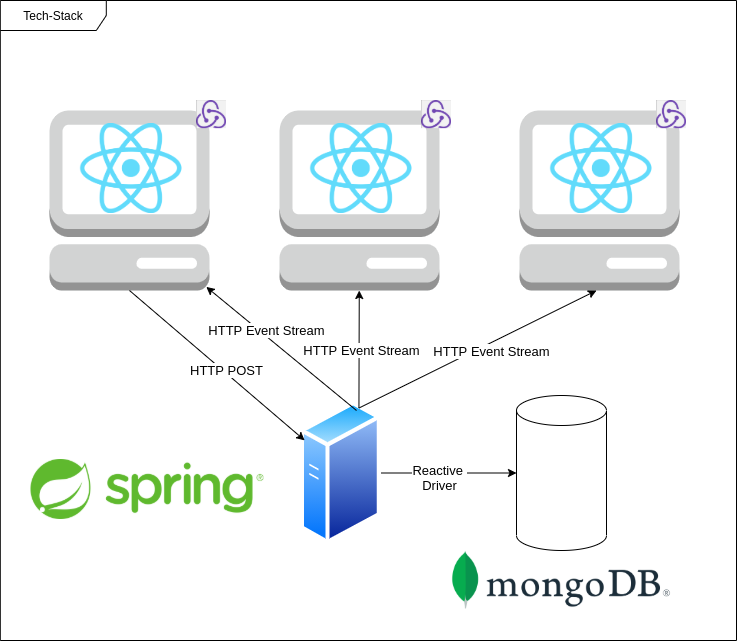
\includegraphics[width=\textwidth,height=\textheight,keepaspectratio]{images/TechStack2.drawio}
    \caption{Technologie Stack}
\end{figure}

\subsection{Applikationsprotokoll}
In der Folge wird auf die verschiedenen Kanäle und das Applikationsprotokoll eingegangen.

\subsubsection{EventSource}
Für die stetige Verbindung der Clients zum Server abonieren die Clients eine EventSource.
Die EventSource ist eine persistente HTTP Verbindung.
Über diese Verbindung hören alle Clients auf Änderungen, die von anderen Clients gemacht werden.
Dieser Kanal sendet alle Kommandos einzeln an die Clients.
Im Fehlerfall wird ein neuer Initial Command ausgelöst, der das gesamte Dokument an alle Clients verteilt.
Damit wird ein konsistenter Zustand erstellt.
Die EventSource wird auch verwendet, um eine Aussage über die verbundenen Clients machen zu können.

\subsubsection{HTTP}
Die Clients wenden im Frontend alle Commands auf sich selber an und senden danach das Command an den Server.
Dafür gibt es einen HTTP POST Endpunkt, der alle Commands entgegen nimmt.
Intern wird anhand des "type" in der Payload entschieden, wie mit dem Command umgegangen wird.

Die genaue Übersicht der Endpunkte ist im Kapitel "API" zu finden.

Der eigentliche Kanal läuft über HTTPS.

\subsubsection{Applikationsprotokoll}
Die Frontend und Backend kommunizieren über JSON.
Jedes JSON Objekt hat folgenden Aufbau:
\begin{itemize}
    \item type: Der Command Type (Bsp. ADD\_PARAGRAPH)
    \item payload: Ein JSON Objekt welches die Payload für den konkreten type enthält
    \item sender: Eine eindeutige ID des Senders
    \item (opt.) correlationId: Eine zufällige, eindeutige ID
\end{itemize}

\subsection{Benutzerverwaltung}
Es ist keine persistente Benutzerverwaltung mit Registrationsprozess implementiert.
Nach erstmaligem Anmelden in der Applikation mit einem globalen Benutzer, wird ein zufälliger Author erstellt.
Die Daten des Authors werden im Local Storage des Browsers gespeichert, sodass bei erneutem Öffnen der Applikation der gleiche Author wiederverwendet wird.

    \section{Frontend}

Das Fronted der TeamDocument Applikation ist als React SPA entwickelt.
Einmal angemeldet kann ein Benutzer an der kollaborativen Bearbeitung des Dokumentes teilnehmen.

Folgende Interaktionen sind möglich:

\begin{itemize}
    \item Ändern des eigenen Namens
    \item Hinzufügen eines neuen Paragrafen
    \item Bearbeitung bestehender Paragrafen
    \item Sperren des Paragrafen an dem gerade gearbeitet wird (implizit)
    \item Verschieben von Paragrafen innerhalb des Dokuments
    \item Löschen eines bestehenden Paragrafen
    \item Wiederherstellen des zuletzt gelöschten Paragrafen (Hidden Feature)
\end{itemize}

Des Weiteren werden folgende Informationen auf dem UI dargestellt:

\begin{itemize}
    \item Name des ursprünglichen Authors eines Paragrafen
    \item Name des Authors welcher aktiv einen Paragrafen bearbeitet.
    \item Highlight des eigenen aktuellen Paragrafen
    \item Liste mit allen Dokumentupdates in chronologischer Reihenfolge
    \item Avatare aller aktiven Benutzer
\end{itemize}

\begin{figure}[H]
    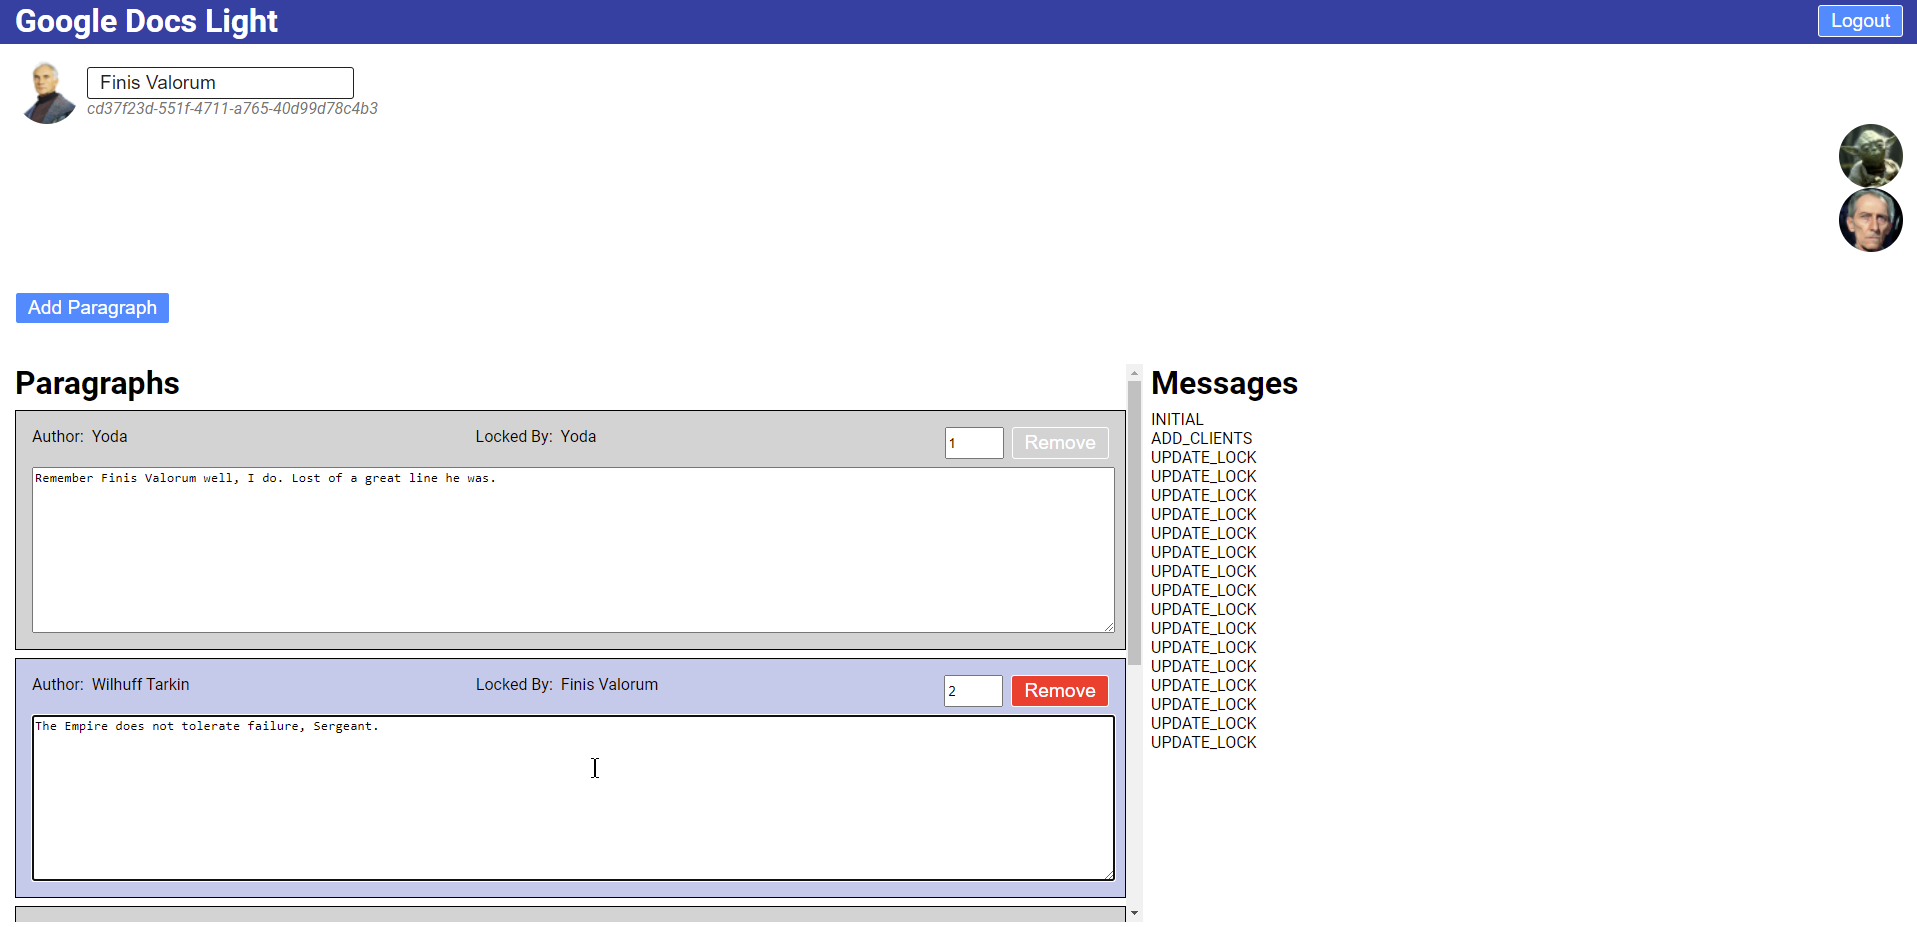
\includegraphics[width=\textwidth,keepaspectratio]{UI-blank}
    \caption{Team Document User Interface}
    \label{fig:Team Document User Interface}
\end{figure}

\subsection{Aufbau}


\subsection{Komponenten}

\begin{figure}[H]
    \centering
    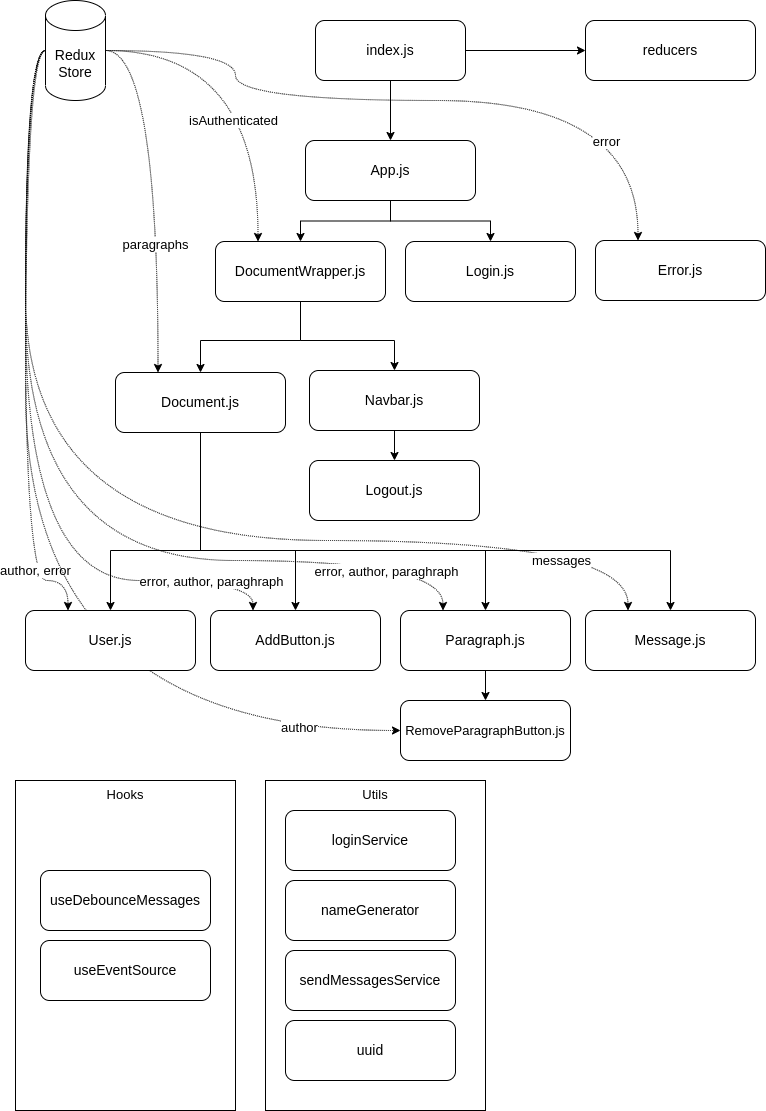
\includegraphics[width=\textwidth,keepaspectratio]{fe_structure}
    \caption{Komponenten Struktur}
    \label{fig: Fe_Structure}
\end{figure}


\begin{figure}[H]
    \centering
    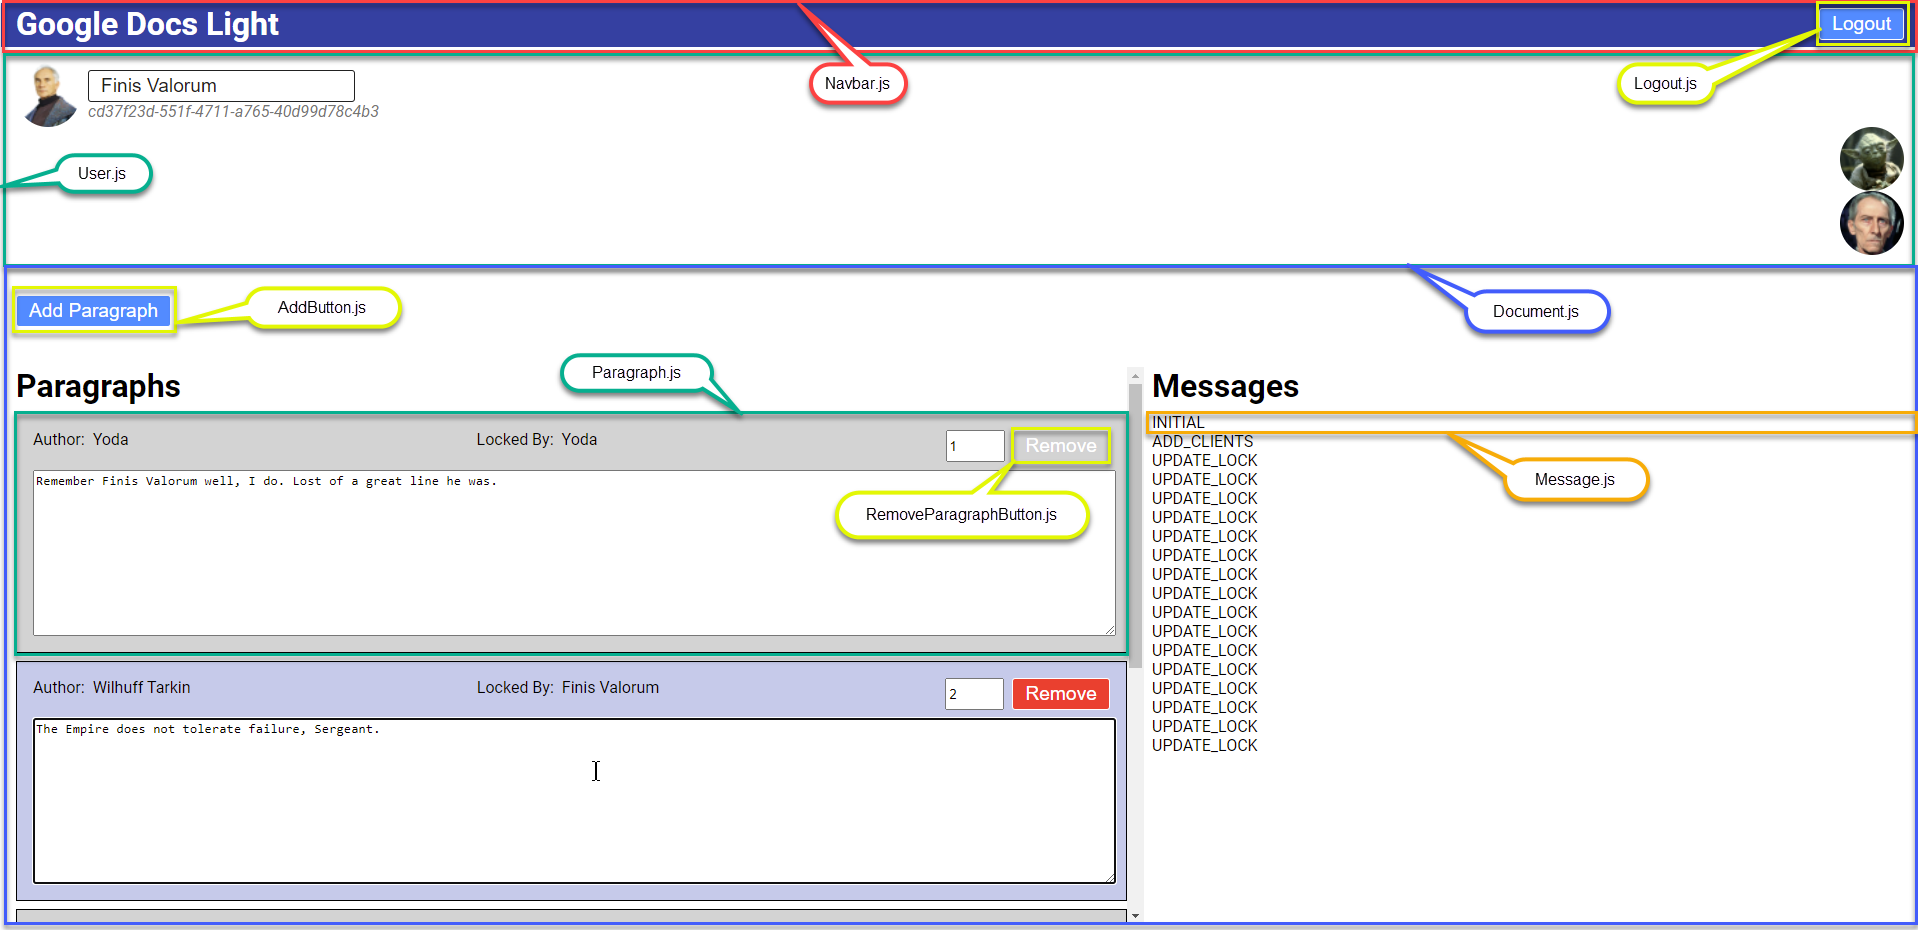
\includegraphics[width=\textwidth,keepaspectratio]{UI-components}
    \caption{UI-Components}
    \label{fig: UI-Components}
\end{figure}

\subsection{Ablaufdiagram}

\begin{figure}[H]
    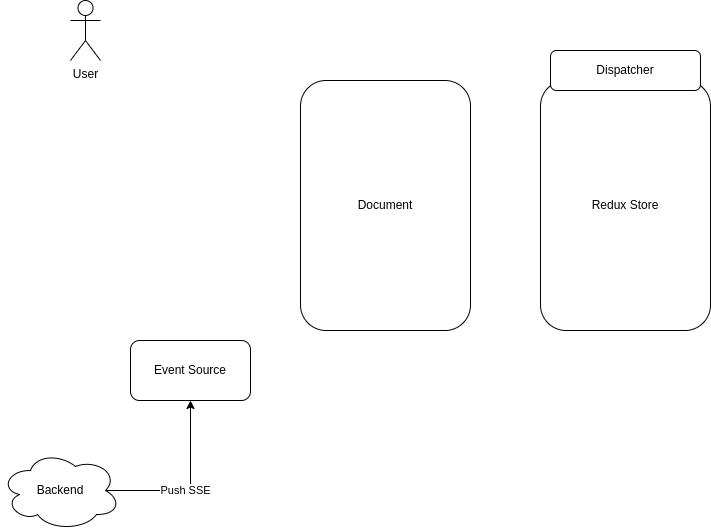
\includegraphics[width=\textwidth,keepaspectratio]{fe_dataflow}
    \caption{Datenfluss}
    \label{fig:}
\end{figure}


\subsection{State- und Konfliktmanagment}
%Redux State Verwaltung

\subsection{Fehler Behandlung}

    \section{Backend}

\subsection{Aufbau}

Der Aufbau der Serverapplikation lehnt sich am Konzept der Onion-Architecture an.
In Onion Architecture wird die Applikation in Layer aufgeteilt.

\begin{figure}[h]
    \centering
    \begin{minipage}[b]{0.4\textwidth}
        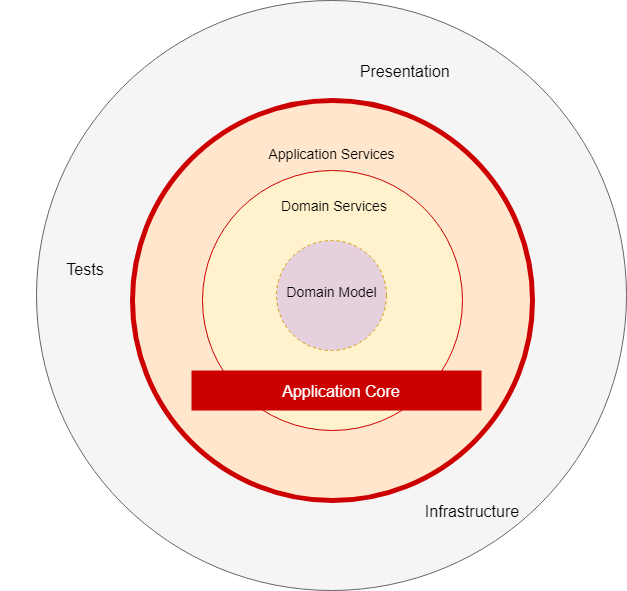
\includegraphics[width=\textwidth]{images/thinktocode-onion}
        \caption{Onion Architecture}
    \end{minipage}\label{fig:figureonion}
\end{figure}

Um zu garantieren, dass keine ungewollten Abhängigkeiten zwischen Layern bestehen, können die Layer in eigene Module verpackt und Abhängigkeiten über Interfaces abstrahiert werden.
Dies erhöht jedoch die interne Komplexität der Applikation.
Die Umsetzung wird aufgrund der geringen Projektgrösse deshalb nicht in unabhängigen Modulen realisiert, sondern über die Packagestruktur gelöst.
Angesichts dieser Entscheidung wird weiter darauf verzichtet, Abhängigkeiten zwischen Modulen über Interfaces zu abstrahieren.
Da es nie mehrere Implementationen einer Komponente geben wird, bringt der Einsatz von Interfaces keinen grossen Mehrwert.
Bei der Implementation wird deshalb konsequent darauf geachtet, die einzelnen Layer so zu halten, dass diese als eigenständige Module extrahiert werden können.
Für die Verwaltung der Komponenten der Serverapplikation wird folgende Packagestruktur definiert:

\begin{figure}[h]
    \centering
    \begin{minipage}[b]{0.9\textwidth}
        \dirtree{%
            .1 ch.fhnw.woweb.teamdocumentserver.
            .2 config.
            .2 domain.
            .2 persistence.
            .2 service.
            .2 web.
        }
        \caption{Packagestruktur Serverapplikation}\label{fig:packagesserver}
    \end{minipage}
\end{figure}

Der Domain Layer wird durch das Package domain abgebildet.
Dieses beinhaltet die Domänenobjekte und darf keine Abhängigkeiten auf andere Module beinhalten.
Umgekehrt dürfen alle anderen Layer Abhängigkeiten auf den Domain Layer haben.
Die Fachlogik der Applikation wird im Domain Service Layer implementiert.
Dieser wird durch das Package Service abgebildet.
Das Package Service beinhaltet alle Komponenten welche die Domänenobjekte verwalten oder den internen Zustand der Applikation führen.
Der Layer Application Services bildet die Brücke zwischen externer Infrastruktur und Domain Services.
Er wird mit den Packages persistence und web abgebildet.
Dabei definiert das Package persistence Services, welche für Interaktion mit der Datenbank verwendet werden.
Das Package web definiert die HTTP-Endpunkte, welche für die Kommunikation mit dem Frontend des Systems verwendet werden.
Letztlich beinhaltet das Package config die technische Konfiguration der Applikation.

\clearpage

\subsection{API}\label{subsec:api}

Die Backendapplikation bietet eine HTTP-Schnittstelle, welche von Frontendapplikationen verwendet werden kann.
Die Schnittstelle ermöglicht es, sich im System anzumelden, Dokumente und Änderungen zu laden und zu speichern.
Um diese Funktionalität zu ermöglichen, bietet die Schnittstelle die drei Bereiche ''Authentication'', ''Document'' und ''Message''.

\subsubsection{API Authentication}

\begin{tabbing}
Left \= Middle \= Right \= Right \kill
Beschreibung:  \> \> \> Authentifizierung mit Basic Auth\\
Endpunkt:  \> \> \> /api/v1/authentication\\
Methode \>  \> \> GET\\
Headers:  \> \>   \> Authentication: Basic \\
Response Code:  \> \>  \> 200, 401 oder 500 \\
Response Body:  \> \>  \> application/json \\
\end{tabbing}

\subsubsection{API Document}

\begin{tabbing}
    Left \= Middle \= Right \= Right \kill
    Beschreibung:  \> \> \> Dokument laden und Updates abonnieren\\
    Endpunkt:  \> \> \> api/v1/document\\
    Methode \>  \> \> GET\\
    Headers:  \> \>   \> Authentication: Basic\\
    \> \>   \> X-ClientId: UUID des Clients als text/plain\\
    Response Code:  \> \>  \> 200, 401 oder 500 \\
    Response Body:  \> \>  \> DocumentCommands als text/event-stream \\
\end{tabbing}


\subsubsection{API Message}

\begin{tabbing}
    Left \= Middle \= Right \= Right \kill
    Beschreibung:  \> \> \> Änderung an Dokument vornehmen\\
    Endpunkt:  \> \> \> /api/v1/message\\
    Methode \>  \> \> POST\\
    Headers:  \> \>   \> Authentication: Basic\\
    \> \>   \> Content-Type: application/json\\
    Body:  \> \>  \> DocumentCommand als application/json\\
    Response Code:  \> \>  \> 200, 401 oder 500 \\
\end{tabbing}

\begin{tabbing}
    Left \= Middle \= Right \= Right \kill
    Beschreibung:  \> \> \> Zuletzt gelöschten Paragraphen wiederherstellen \\
    Endpunkt:  \> \> \> /api/v1/message/restore\\
    Methode \>  \> \> POST\\
    Headers:  \> \>   \> Authentication: Basic\\
    Response Code:  \> \>  \> 200, 401 oder 500 \\
\end{tabbing}

\begin{tabbing}
    Left \= Middle \= Right \= Right \kill
    Beschreibung:  \> \> \> Dokument zurücksetzen \\
    Endpunkt:  \> \> \> /api/v1/message/reset\\
    Methode \>  \> \> DELETE\\
    Headers:  \> \>   \> Authentication: Basic\\
    Response Code:  \> \>  \> 204, 401 oder 500 \\
\end{tabbing}

\clearpage

\subsection{Komponenten}\label{subsec:komponenten}

\subsubsection{Package Domain}

Abbildung 4.3 zeigt die Klassen, des Packages Domain.
Sämtliche Klassen in diesem Package besitzen einen öffentlichen Konstruktor, welcher für alle Instanzvariablen einen Parameter entgegennimmt.
Diese Konstruktoren sind in der Abbildung nicht abgebildet.
Im Zentrum der Domäne stehen die beiden Klassen DocumentCommand und Document.

\begin{figure}[h]
    \centering
    \begin{minipage}[b]{0.8\textwidth}
        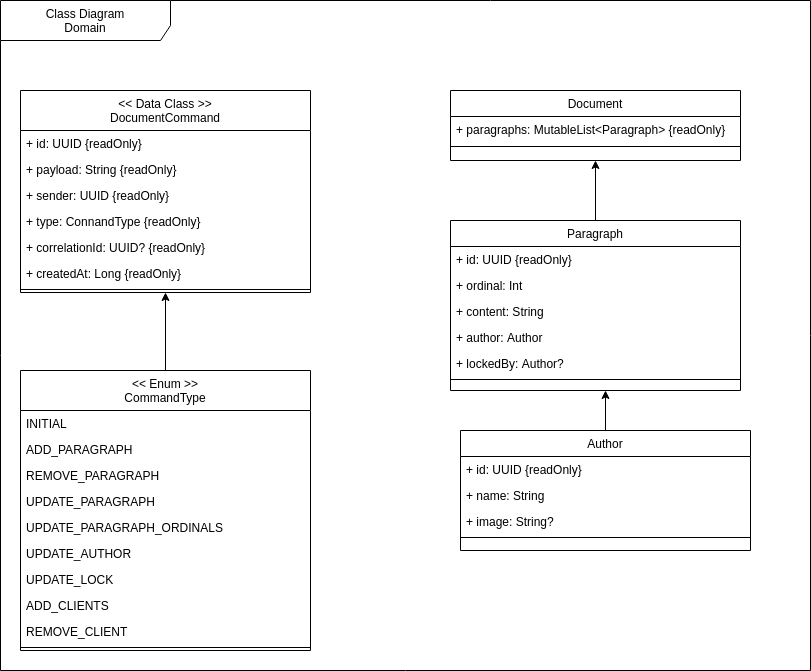
\includegraphics[width=\textwidth]{images/class-be-domain.drawio}
        \caption{Klassendiagramm Domain}
    \end{minipage}
\end{figure}

\textbf{Document}

Eine Instanz der Klasse Document repräsentiert den aktuellen Zustand eines Dokuments.
Dieser Zustand wird in der Serverapplikation geführt und verwaltet.
Ein Document besteht im Wesentlichen aus einer Liste von Paragraphs.
Diese Liste kann mutiert, aber nicht ersetzt werden.

\textbf{Paragraph}

Eine Instanz der Klasse Paragraph repräsentiert einen Abschnitt in einem Dokument.
Jeder Paragraph wird durch eine UUID identifiziert und ist einem Autor zugewiesen.
Ein Paragraph definiert weiter ein Attribut ''content'',  welches den Textinhalt des Abschnitts beinhaltet und ein Attribut ''ordinal'', welches die Position des Abschnitts im Dokument darstellt.
Letztlich hat ein Paragraph ein Optionales Attribut ''lockedBy''.
Dieses kann entweder leer (NULL) sein oder einen Autor beinhalten.
Dieses Feld kann von Consumern der API verwendet werden, um das bearbeiten eines Paragraphen zu erlauben oder verbieten.

\textbf{Author}

Eine Instanz der Klasse Author repräsentiert einen Benutzer, der an einem Dokument mitarbeitet.
Jeder Author wird durch eine UUID identifiziert und muss einen Namen definieren.
Weiter besitzt ein Author ein optionales Attribut ''image''.
Darin kann die URL zu einem Benutzerbild abgespeichert werden

\clearpage

\textbf{DocumentCommand}

Eine Instanz der Klasse DocumentCommand stellt eine Änderung am Zustand einer Document-Instanz dar.
DocumentCommands werden als einzige Entität persistiert.
Damit DocumentCommands eindeutig identifiziert werden können, beinhaltet jede Instanz ein Attribut ''id'' vom Typ UUID\@.
Diese id wird auch als Identifikator in der MongoDB verwendet.

Die Änderungen welche ein DocumentCommand darstellt, werden über die Attribute ''payload'' und ''type'' definiert.
Die Payload hat den Typ String und beinhaltet JSON-serialisierte Daten, welche die vorzunehmenden Änderung darstellen.
Das Feld ''type'' beinhaltet einen Wert aus der Enum CommandType.
Dieser Wert kann in den Serviceklassen verwendet werden, um die Payload korrekt zu deserialisieren und die nötigen Änderungen am Dokument vorzunehmen.

Das Optionale Feld ''correlationId'' kann entweder NULL oder eine UUID beinhalten.
Eine allfällige UUID zeigt immer auf die Id eines anderen DocumentCommands, welcher mit dem aktuellen Command zusammenhängt.
Dadurch wird es möglich, die Identifkation der Payload eines Commands zu verwenden, ohne die Payload deserialisieren zu müssen.

\textbf{CommandType}

Bei CommandType handelt es sich um eine Enum.
Diese Enum beinhaltet alle Arten von DocumentCommands, welche im System bekannt sind.
CommandTypes werden als ihr String Wert auf DocumentCommands persistiert.
Der verwendete CommandType bestimmt, wie ein Command verarbeitet wird.
Dies ist in Kapitel 4.5 weiter beschrieben.

\subsubsection{Package Web}

\textbf{AuthenticationController}

Die Klasse AuthenticationController implementiert einen Spring RestController.
Dieser stellt einen einzelnen GET-Endpunkt zur Verfügung, über welchen sich Benutzer mittels Basic Authentication anmelden können.

\textbf{CommandController}

Die Klasse CommandController implementiert einen Spring RestController.
Dieser Controller stellt zwei POST-Endpunkte zur Verfügung.
Über den ersten Endpoint kann eine Liste von DocumentCommands an den Server gesendet werden.
Der Endpunkt übergibt diese Liste von Commands an den DocumentService.
Diese wenden die Änderungen am Zustand des Dokuments an und leiten die Änderungen an andere Teilnehmer weiter.
Über den zweiten Endpunkt kann ein gelöschter Paragraph wiederhergestellt werden.
Die entsprechende Fachlogik wird an den DocumentService delegiert.
Letztlich stellt der Controller einen DELETE-Endpunkt zur Verfügung.
Über diesen kann der Zustand des Dokuments zurückgesetzt werden.

\textbf{DocumentStreamUpdateController}

Die Klasse DocumentStreamUpdateController implementiert einen Spring RestController.
Dieser Controller ermöglicht es, den aktuellen Zustand eines Dokumentes zu laden und Änderungen am Dokument zu abonnieren.
Der Endpunkt, welcher dazu zur Verfügung steht erwartet, dass der Custom Header ''X-ClientId'' gesetzt ist.
Dieser muss einen die Id des Authors, der die Daten laden möchte, beinhalten.
Das Laden des Dokuments und das Erstellen der Abonnierung wird an den DocumentService delegiert.
Als Rückgabetyp wird ''Flux$<$DocumentCommand$>$'' verwendet.
Dadurch ist es möglich den Status des Documents und alle folgenden Änderungen in einem Stream zurückzugeben.

\clearpage

\subsubsection{Package Services}

\begin{figure}[h]
    \centering
    \begin{minipage}[b]{0.8\textwidth}
        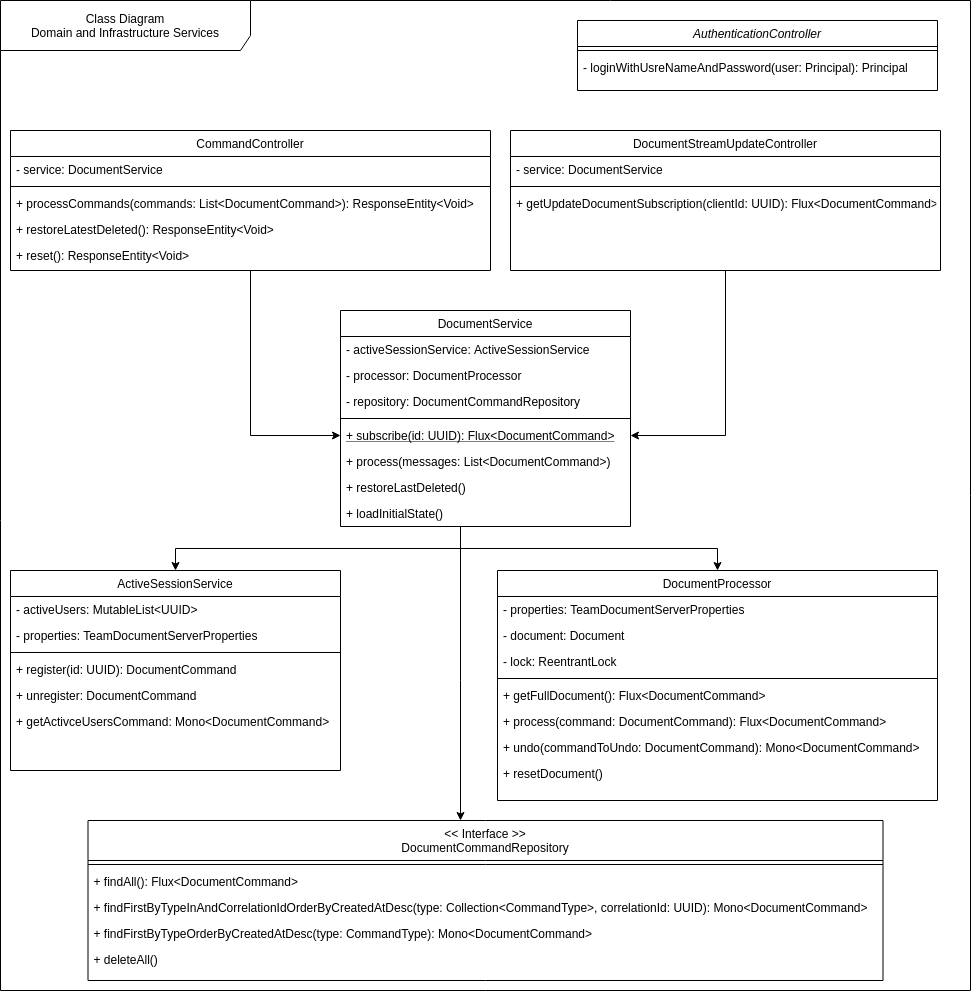
\includegraphics[width=\textwidth]{images/class-be.drawio}
        \caption{Klassendiagramm Services}
    \end{minipage}
\end{figure}


\textbf{DocumentService}

Die Klasse DocumentService ist dafür verantwortlich, erhaltene Anfragen für Dokumente und Änderungen an Dokumenten zu verarbeiten.
Sie delegiert die entsprechende Fachlogik an die Klassen ActiveSessionService, DocumentProcessor und DocumentCommandRepository.

Die Methode process erlaubt es, eine Liste von DocumentCommands zu verarbeiten.
Die Methode subscribe erlaubt es, einen Stream des aktuellen Zustands des Dokuments und aller künftigen Änderungen an einem Dokument anzufragen.
Beide Abläufe werden in Kapitel 4.4 beschrieben.

\textbf{DocumentProcessor}

Die Klasse DocumentProcessor führt den Zustand des Dokuments, welches mit der Applikation verwaltet wird.
Er ist dafür Verantwortlich, Änderungen an diesem Dokument vorzunehmen.
Dazu besitzt Sie ein privates Attribut document vom gleichnamigen Typ.
Über die Methode process kann ein einzelner DocumentCommand angewendet werden.
Der Processor verarbeitet den Command anhand des gesetzten CommandTypes.
Dabei muss er allfällige Konflikte erkennen und auflösen.
Nach der Verarbeitung des Commands werden alle Änderungen und Konfliktlösungen als DocumentCommands zurückgegeben.
\clearpage
\textbf{ActiveSessionService}

Die Klasse ActiveSessionService führt den Zustand der aktiven Nutzer einer Session.
Dazu führt die Klasse eine Liste der Identifikatoren aller aktiven Nutzer.
Der Service bietet Methoden um die aktiven Benutzer auszulesen, einen neuen Benutzer zu registrieren und einen Benutzer zu entfernen.

\subsubsection{Package Persistence}

\textbf{DocumentCommandRepository}

Das Interface DocumentCommandRepository erweitert das Interface ReactiveCrudRepository von Spring.
Es kann damit verwendet werden um Create, Read, Update und Delete Optionen für DocumentCommands in der angebundenen MongoDB auszuführen.

\subsubsection{Konfiguration}

\textbf{Spring}

Alle Klassen im Package ''Service'' sind mit der Spring-Boot-Annotation ''@Service'' versehen.
Sie können damit automatisch von Spring-Boot instanziiert werden und stehen Sie in Spring Beans zur Verfügung und können über Constructor-Injection verwendet werden.

Alle Klassen im Package ''web'' sind mit der Spring-Boot-Annotation ''@RestController'' versehen.
Sie können damit automatisch von Spring-Boot instanziiert werden.

\textbf{application.yml}

Die Datei application.yml beinhaltet die konfigurierbaren Werte der Serverapplikation.
Dies beinhaltet die Konfiguration der angebundenen MongoDB, Referenzen zu Umgebungsvariablen mit User Credentials und Logging Konfiguration.

\textbf{TeamDocumentServerProperties}

Die Konfigurationsklasse TeamDocumentServerProperties ist mit der Annotation ''@ConfigurationProperties(prefix = "teamdocument")'' versehen.
Sie kann in den Serviceklassen verwendet werden, um auf Werte aus dem application.yaml zuzugreifen.

\textbf{WebConfig}

Die Klasse WebConfig beinhaltet die Konfiguration für SpringSecurity.

\clearpage

\subsection{Abläufe}

\subsubsection{Dokument laden und Änderungen abonnieren}

\begin{figure}[h]
    \centering
    \begin{minipage}[b]{1\textwidth}
        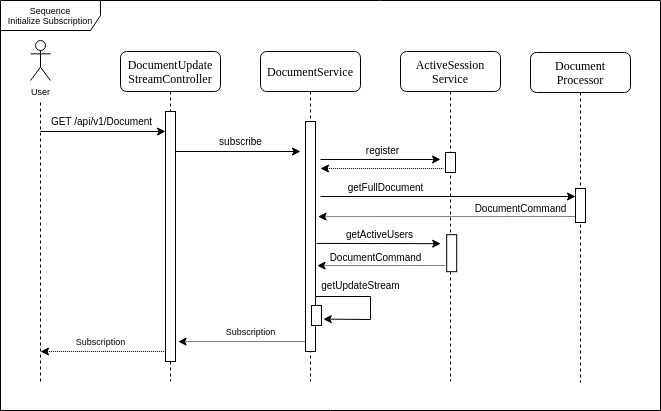
\includegraphics[width=\textwidth]{images/seq_init_subscription.drawio}
        \caption{Sequenzdiagramm Document Subscription}
    \end{minipage}\label{fig:figureseqsub}
\end{figure}

Die Komponente DocumentUpdateStreamController erlaubt es, ein Dokument zu laden und Änderungen an diesem Dokument zu abonnieren.
Dazu bietet der RestController einen Endpunkt, welcher ein Resultat vom Typ Flux$<$DocumentCommand$>$ zurückgibt.
Nachdem eine Anfrage beim Controller eingegangen ist, delegiert dieser die Erstellung des Flux an den DocumentService.
Dieser registriert den Client hinter der Subscription beim ActiveSessionService und trägt anschliessend Informationen aus drei Quellen zusammen.
Zuerst wird der aktuelle Stand des Dokuments beim DocumentProcessor angefragt.
Anschliessend wird eine Liste aller aktiven Clients des Dokuments aus dem ActiveSessionService geladen.
Letztlich wird eine Subscription für Änderungen am Dokument erstellt.
Der DocumentService führt dazu eine Instanzvariable vom Typ Sink.
Alle Änderungen werden nach der Anwendung in diesen Sink geschrieben.
Eine Subscription auf diesem Sink beinhaltet damit alle Änderungen, welche vorgenommen wurden.
Die Informationen zum initialen Stand des Dokuments, aktiven Clients und die Subscription auf Änderungen werden in einem einzelnen Flux zusammengefasst und zurückgegeben.
Nachdem der Flux geschlossen wird, wird die Registrierung des aktiven Benutzers im ActiveSessionService wieder entfernt.

\subsubsection{Änderungen verarbeiten}

Die Komponente CommandController erlaubt es, Änderungen an einem Dokument vorzunehmen und zu persistieren.
Der Controller bietet dazu einen HTTP-Endpunkt, über welchen ein JSON-serialisierter DocumentCommand übergeben werden kann.
Ein DocumentCommand definiert unter anderem einen Typ, welcher ein Wert der Enum CommandType sein muss und eine Payload vom Typ String.
Die Payload ist wiederum ein JSON-serialisiertes Objekt.
Die Verarbeitung eines DokumentCommands wird vom Controller an den DocumentService delegiert.
Dieser übergibt den Command wiederum an den DocumentProcessor.
Dieser wendet Änderungen an und löst Konflikte auf.
Die übergebenen Commands und allfällige Commands zur Konfliktlösung werden vom DocumentProcessor zurückgegeben.
Der DocumentService übergibt diese an das DocumentCommandRepository zur Persistierung in der Datenbank.
Anschliessend werden die persistierten Commands über die Instanzvariable vom Typ Sink veröffentlicht.
Registrierte Clients haben eine Subscription auf diesen Sink und werden so über die Änderungen informiert.

\begin{figure}[h]
    \centering
    \begin{minipage}[b]{1\textwidth}
        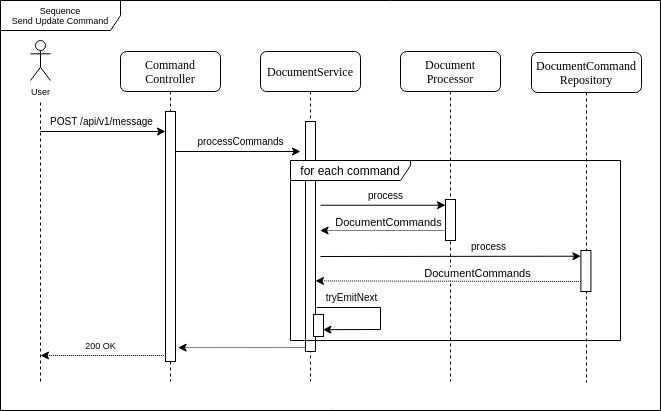
\includegraphics[width=\textwidth]{images/seq_send_command.drawio}
        \caption{Sequenzdiagramm Command verarbeiten}
    \end{minipage}\label{fig:figuresqcmd}
\end{figure}

\subsubsection{Fehlerbehandlung}

Fachliche Fehler, die während der Verarbeitung von Änderungen an einem Dokument auftreten, werden innerhalb des DocumentProcessors behandelt.
Dabei werden immer zusätzliche Änderungen generiert, welche Konflikte lösen.
Die Verarbeitung wird nie durch das Werfen von Exceptions unterbrochen.
Es ist möglich, dass die Verarbeitung einer Änderung oder das Veröffentlichen von Änderungen wegen einem technischen Fehler fehlschlägt.

Wenn eine Exception beim Verarbeiten einer Änderung auftritt, wird die Verarbeitung abgebrochen und die Exception weiter geworfen.
Exceptions werden in den Controller Klassen abgefangen.
Im Fehlerfall wird dort die Exception in das Log geschrieben und eine ResponseEntity mit Statuscode 500 zurückgegeben.

Wenn eine Exception beim Veröffentlichen einer Änderung auftritt, wird die Subscription geschlossen.
Dadurch wird die Verbindung des betroffenen Clients getrennt.
Es liegt in der Verantwortung des Clients die Verbindung erneut zu öffnen und den aktuellen Stand des Dokuments zu laden.

\clearpage

\subsection{Zustands- und Konfliktmanagement}\label{subsec:statemgmt}

Um sicherzustellen, dass ein Dokument auf allen Clients einen konsistenten Zustand hat, wird der Zustand des Dokuments in der Serverapplikation geführt.
Änderungen von Clients müssen an den Server gesendet werden.
Dieser wendet die Änderungen auf dem Dokument an und leitet die Änderungen an alle anderen Clients weiter.
Während der Anwendung von Änderungen, ist es in der Verantwortung der Serverapplikation, sicherzustellen, dass das Dokument in einem Konsistenten Zustand bleibt.
Wenn nötig, erstellt es dazu zusätzliche Änderungen und veröffentlicht diese ebenfalls an alle Clients.

Die entsprechende Fachlogik ist in den Klassen DocumentService und DocumentProcessor implementiert.
Dabei ist die Klasse DocumentProcessor für die Zustandsverwaltung des Dokuments verantwortlich.


\subsubsection{Grundsatz}

Der DocumentProcessor hat zwei private Instanzvariablen, die für das Zustandsmanagement relevant sind.
Die Variable \textbf{document} ist vom gleichnamigen Typ.
Diese Document-Instanz stellt die ''Source Of Truth'' für den Zustand des Dokuments dar.
Ein Document besteht im Wesentlichen aus einer Liste von Paragraphen.
Diese Liste wird mit ''synchronizedList(mutableListOf<Paragraph>())'' initialisiert.
Dadurch wird sichergestellt, dass der Zugriff für die Liste zwischen der Verarbeitung einzelner Commands synchronisiert ist.
Die Variable \textbf{lock} hat den Typ ReentrantLock.
Die Verarbeitung einiger DocumentCommands darf nicht parallel passieren, weil dadurch Konflikte ausgelöst werden können.
Die Verarbeitung solcher DocumentCommands wird durch die Verwendung dieses ReentrantLocks gesperrt.

\subsubsection{Zustandsänderungen}

Alle Änderungen werden als Instanzen der Klasse DocumentCommand an den Server übermittelt.
Nachfolgend wird beschrieben, welche Arten von DocumentCommands unterstützt sind, wie diese verarbeitet werden und wie mit möglichen Konflikten umgegangen wird.

Ein DocumentCommand mit Typ \textbf{INITIAL} stellt den vollständigen Zustand eines Dokuments dar.
Er beinhaltet als Payload eine Liste der Paragraphen in diesem Dokument.
INITIAL Commands werden im Backend generiert, um den vollständigen Zustand eines Dokuments zu veröffentlichen.
Eingehende INITIAL Commands werden im DocumentProcessor nicht angewendet.

Ein DocumentCommand mit Typ \textbf{ADD\_PARAGRAPH} fügt einen neuen Abschnitt zum Dokument hinzu.
Er beinhaltet als Payload einen einzelnen Paragraphen.
Dieser Paragraph wird im DocumentProcessor deserialisiert und der Liste von Paragraphen im Dokument hinzugefügt.
Es ist möglich, gleichzeitig zwei Commands eingehen, welche an derselben Stelle im Dokument einen Paragraphen einfügen möchten.
Deshalb wird hier sichergestellt, dass die Ordinalnummern aller Paragraphen korrekt sind und keine Nummer doppelt vorkommt.
Während diese Korrektur vorgenommen wird, dürfen keine anderen Änderungen möglich sein.
Deshalb wird die Verarbeitung eines ADD\_PARAGRAPH Commands mit dem ReentrantLock versehen.
Nach der Verarbeitung werden die ADD\_PARAGRAPH und UPDATE\_PARAGRAPH\_ORDINALS Commands zurückgegeben, damit Sie veröffentlicht werden können.

Ein DocumentCommand mit Typ \textbf{REMOVE\_PARAGRAPH} entfernt einen Paragraphen aus dem Dokument.
Ein beinhaltet als Payload die UUID, des zu entfernenden Abschnitts.
Bei der Verarbeitung wird der Abschnitt mit der gegebenen Id entfernt.
Ist der Abschnitt bereits entfernt, wird kein Fehler geworfen.
Nachdem ein Paragraph entfernt wurde, muss sichergestellt werden, dass es keine Lücke in den Ordinal Nummern der Paragraphen gibt.
Deshalb wird auch hier sichergestellt, dass die Ordinalnummern aller Paragraphen korrekt sind.
Anschliessend werden die REMOVE\_PARAGRAPH und UPDATE\_PARAGRAPH\_ORDINALS zurückgegeben.
Um sicherzustellen, dass die Ordinalnummern korrekt gesetzt werden, ist auch diese Verarbeitung mit dem ReentrantLock abgeschlossen.

Ein DocumentCommand mit Typ \textbf{UPDATE\_PARAGRAPH} aktualisiert den Textinhalt eines Abschnitts.
Er beinhaltet als Payload einen einzelnen Paragraphen.
Bei der Verarbeitung wird der relevante Abschnitt im Dokument gefunden und dessen Inhalt überschrieben.
Hier wird bewusst kein explizites Konfliktmanagement betrieben.
Paragraphen dürfen nur bearbeitet werden, wenn der Benutzer den Paragraph für sich gesperrt hat.
Da ein Paragraph immer nur von einem Benutzer gesperrt sein kann und Updates in derselben Reihenfolge wie sie geschehen eingehen, können diese Updates immer angewendet werden.
Es ist möglich, dass sich das Sperren eines Pargraphen von zwei Benutzern überschneidet.
Am Ende darf aber immer nur ein Benutzer den Paragraphen gesperrt haben.
In diesem Fall ist es das gewünschte Verhalten, dass die Änderungen dieses Benutzers alle anderen Änderungen am selben Abschnitt überschreiben. 

Ein DocumentCommand mit Typ \textbf{UPDATE\_PARAGRAPH\_ORDINALS} aktualisiert die Ordinalnummern von Abschnitten.
Er beinhaltet als Payload eine Liste von Paragraphen.
Bei der Verarbeitung dieses Commands werden die Ordinalnummern aller Abschnitte mit den Ordinalnummern aus der Payload überschrieben.
Anschliessend wird sichergestellt, dass die Ordinalnummern aller Paragraphen korrekt sind und keine Nummer doppelt vorkommt.
Es werden darauf der erhaltenen Command und Commands zur Konfliktlösung zurückgegeben.
Um sicherzustellen, dass die Ordinalnummern korrekt gesetzt werden, ist auch diese Verarbeitung mit dem ReentrantLock abgeschlossen.

Ein DocumentCommand mit Typ \textbf{UPDATE\_AUTHOR} aktualisiert den Namen eines Authors, der das Dokument bearbeitet.
Er beinhaltet als Payload eine Author-Instanz.
Der Name dieses Authors wird auf allen Abschnitten im Dokument aktualisiert.
Anschliessend wird der Command zurückgegeben.
Es wird hier kein explizites Konfliktmanagement betrieben, da ein Benutzer immer nur an genau einem Gerät arbeiten kann.
Sollte derselbe Benutzer auf mehreren Clients verwendet werden und gleichzeitig den Namen ändern, können sich diese Änderungen überschreiben.
In diesem Fall wird das zuletzt gesendete Update angewendet und veröffentlicht.
Damit ist der Zustand auch bei Konflikten konsistent.

Ein DocumentCommand mit Typ \textbf{UPDATE\_LOCK} erlaubt es einen Abschnitt durch einen Benutzer zu ent-/sperren.
Dies wird in den Clients verwendet, um sicherzustellen, dass nur ein Benutzer gleichzeitig an einem Paragraph arbeiten kann.
Die Payload dieses Commands beinhaltet als Payload den Pargraphen, der gesperrt werden soll.
Dieser Paragraph wird in der Liste von Pargraphen gefunden und durch setzten des lockedBy Attributs gesperrt.
Ist auf der Payload kein lockedBy Attribut gesetzt, wird die Sperre entfernt.
Dabei wird sichergestellt, dass eine Sperre nur durch den Benutzer, der sie erstellt hat entfernt werden kann.
Versucht ein anderer Benutzer, die Sperre aufzuheben, wird die Verarbeitung abgebrochen und ein Command welcher die Sperre zurücksetzt zurückgegeben.
Damit sich das Sperren von Paragraphen zwischen Benutzern nicht überschneiden kann, ist die Verarbeitung dieses Commands mit dem ReentrantLock versehen. 

Ein DocumentCommand mit Typ \textbf{ADD\_CLIENTS} teilt mit, dass ein neuer Bearbeiter am Dokument existiert.
Dieser Command führt zu keiner Änderung am Dokument und wird im DocumentProcessor nicht verarbeitet.
Er wird bei der Registrierung einer Subscription erstellt und veröffentlicht.

Ein DocumentCommand mit Typ \textbf{REMOVE\_CLIENT} teilt mit, dass die Verbindung eines Bearbeiters getrennt wurde.
Bei der Verarbeitung dieses Commands werden alle Paragraphen, welche durch diesen Bearbeiter gesperrt waren entsperrt.
Dadurch wird sichergestellt, dass Paragraphen nicht gesperrt sind wenn ein Benutzer den Client beendet oder die Verbindung abbricht.
Der Command wird durch den ActiveSessionService generiert und vom DocumentProcessor verarbeitet, nachdem ein Client die Verbindung getrennt hat.

\clearpage

    \section{Testing}

Das Testing der Applikation soll einerseits Unit Tests in Frontend und Backend beinhalten, sowie Integration Tests, die das Verhalten der kompletten Applikation \"uberpr\"ufen.
Eine der identifizierten Problemquellen ist das Netzwerk.
Dieses wird aber nicht explizit weiter getestet oder simuliert, da es kein Teil der Nutzererfahrung ist, die wir beeinflussen k\"onnen.
F\"ur die einzelnen Teile der Applikation sollen Testframeworks angewandt werden, die grosse Verwendung finden und f\"ur die ausgew\"ahlte Technologie \"ublich ist.

\subsection{Frontend}
F\"ur das Frontend wird Jest \url{https://jestjs.io/} verwendet.

Jest folgende Vorteile:

\begin{enumerate}
    \item Integration f\"ur React und Babel
    \item Einfachheit
    \item Ohne Browser ausf\"uhrbar
    \item Einfach aufzusetzen
    \item Schnell in der Ausf\"uhrung und dem Feedback
\end{enumerate}

Es sollen einzelne Komponenten getestet werden, damit deren Funktionalit\"at gegeben ist.
Es wird darauf verzichtet Enzyme als zus\"atzliche Dependency einzubinden, da die Tests einfach gehalten werden sollen.
Da die einzelnen Komponenten oftmals nur Kommandos an Redux dispatchen, ist deren Testing als abgeschottete Komponente nicht immer zielf\"uhrend, da indirekt die Funktionalit\"at von Redux getestet wird.
Es bietet sich deshalb an, mehrere Funktionen in die End to End Tests zu verschieben.

\subsection{Backend}

\subsubsection{Unit Tests}

Sämtliche Service- und Controller Klassen werden mit Unit-Tests getestet.
Dazu wird das Framework JUnit verwendet.
Die Unit Tests testen jeweils genau eine Klasse.
Sämtliche Abhängigkeiten auf andere Services werden mit dem Framework Mockito gemocked.

\subsubsection{Lasttests}

Neben den einfachen Unit Tests wurden für den DocumentProcessor Lasttests implementiert.
Diese stellen sicher, dass der DocumentProcessor Änderungen auch unter grössere Last schnell verarbeitet und dabei einen konsistenten Zustand im Dokument erstellt.
In diesen Lasttests werden drei Benutzer simuliert welche parallel je 512 DocumentCommands verarbeiten lassen.
Dabei wird vor jedem Verarbeitungsschritt eine zufällige Verzögerung von max. einer Sekunde eingebaut.
Der Test stellt sicher, dass im Schnitt nicht mehr als vier Millisekunden für die Verarbeitung eines Commands verwendet.
Der Test prüft weiter, dass das Dokument nach der Verarbeitung den erwarteten Zustand hat.

\subsubsection{Application Tests}

Mit der Testklasse TeamDocumentServerApplicationTests wird die Backendapplikation als Ganzes getestet.
Dazu wird der gesamte Application Context hochgefahren.
Anschliessend werden DocumentCommands direkt über die Controller Klassen verarbeitet.
Dabei wird geprüft, dass Änderungen korrekt angewendet und veröffentlicht werden.

In den Application Tests werden zudem einfache Lasttests ausgeführt.
Gleich wie bei den Lasttests auf dem DocumentProcessor werden hier drei Benutzer simuliert welche parallel je 512 DocumentCommands verarbeiten lassen.
Anschliessend wird sichergestellt, dass im Schnitt nicht mehr als 40 Millisekunden für die Verarbeitung eines Commands verwendet wird.
Es wird weiter geprüft, dass das Dokument nach der Verarbeitung in einem Konsistenten zustand ist.



\subsection{End to End Test}
F\"ur das End to End Testing wird Cypress verwendet.

Cypress bietet folgende interessanten Features:

\begin{enumerate}
    \item Simulation eines Browsers
    \item DOM Traversierung anhand von CSS Selektoren
    \item \"Uberpr\"ufen von Attributen, CSS Klassen, Value, \ldots
    \item Aufnehmen von Test Cases mittels experimentellen Features im Cypress Studio
\end{enumerate}

Cypress bietet aber explizit ein wichtiges Feature nicht: Es ist nicht m\"oglich mehrere Tabs oder Browser Fenster zu simulieren.
Aus \url{https://docs.cypress.io/guides/references/trade-offs}: "There will never be support for multiple browser tabs."

Konkret bedeutet dies f\"ur das Testing der Applikation, dass nicht mehrere Nutzer mit Cypress simuliert werden k\"onnen.
Um dem entgegenzuwirken, wird eine Klasse f\"ur einen Dummy User geschrieben, der direkt die API der Applikation ansteuert.
Mehrere Instanzen dieser Klasse k\"onnen somit die Multiuser Interaktion simulieren.
Damit kann getestet werden, dass der maschinell gesteuerte Anwender von Cypress einen konsistenten Zustand beim Arbeiten antrifft.
Auch f\"ur andere Basis Funktionen wie das Locking ist es notwendig mehrere Nutzer einzubringen.

Da die End to End Test auf die Datenbank zugreifen, ist es ebenfalls notwendig einen Endpunkt anzubieten, der den Zustand des Dokuments zwischen den Ausf\"uhrungen zur\"ucksetzt.

\subsubsection{Probleme}
Nebst der angesprochenen Einzelnutzer Limitierung gibt es noch andere Herausforderungen im Zusammenhang mit dem End to End Testing.
Da jedes Update ein eigenes Kommando erzeugt, kann es es sein, dass Cypress beispielsweise zu schnell tippt und bereits die n\"achste Aktion ausf\"uhrt, bevor das Backend die Inputs verarbeiten konnte.
Beim normalen Arbeiten mit dem Dokument w\"urde einfach der letzte konsistente Zustand hergestellt.
Beim Test ist es aber notwendig, dass von einem Bestimmten Output oder Status in der Applikation ausgegangen werden kann, um die Testbedingung zu erf\"ullen.
Damit dies beim Testen nicht zum Problem wird, werden \"ofters cy.wait() Statements und delay Optionen auf Input aufgerufen.
Dies ist aus Sicht des Testings vertretbar, da ein Mensch auch einen Abstand zwischen einzelnen Tastenanschl\"agen hat, eine "Think Time" hat oder auch auf das visuelle Feedback der Applikation warten kann.
Einzelne cy.wait() Statements werden beispielsweise verwendet, um das Laden der Applikation nach dem Login oder das Zur\"ucksetzen des Dokuments abzuwarten.

\subsubsection{Stress Tests}
Die Stress Tests werden mit mehreren Instanzen der User Klasse ausgef\"uhrt.
Der "User" verwaltet dabei einen eigenen State seiner Paragraphen in Memory und ruft die API auf, um seine eigenen Paragraphen im Dokument zu ver\"andern.
Der Cypress User interagiert mit diesen anderen Usern und versucht dabei seine Aufgaben abzuarbeiten.

Stress Tests auf dem Live System wurden unsystematisch w\"ahrend der Entwicklung durch die Entwickler mit mehreren Browsern ausgef\"uhrt.
Dadurch konnten jedoch verschiedene Probleme festgestellt werden, wie zum Beispiel die Limitierung \"uber das Netzwerk oder die Notwendigkeit eines gr\"osseren Buffers.
    \section{Deplyoment}

Die Applikation ist auf einen virtuellen Ubuntu Server bei Switch Tube deployt.
Für Frontend und Backend sind eigene Docker Images erstellt.
Für die Datenbank verwenden wir das Offizielle MongoDB Image.
Die Container werden mit Docker-Compose verwaltet.

\subsubsection*{Frontend}
Das Frontend-Image wird mit einem Multi-Stage Dockerfile gebaut.
Der Builder ist ein Node Container welcher den Production-Build erstellt.
Diese Artefakte werden in einen NGINX Container kopiert.

NGINX dient dabei als Webserver für das Frontend und gleichzeitig als Reverse-Proxy.
Alle API Anfragen werden so durch den NGINX Server entgegengenommen und zum internen Dockernetzwerk weitergeleitet.

\subsubsection*{Backend}
Der Spring Server wird auf Basis des OpenJdk 11 Images gebaut.
Spring Webflux verwendet per Default den Reactor Netty Webserver.
Die Anbindung zur MongoDB ist direkt in den Application Properties konfiguriert.


\subsubsection*{Protokolle}
Gegen die Öffentlichkeit präsentiert der NGINX Webserver TLS Zertifikate von Let's Encrypt.
Alle eingehenden HTTP Anfragen auf Port 80 werden weitergeleitet nach Port 443.


\begin{figure}[H]
    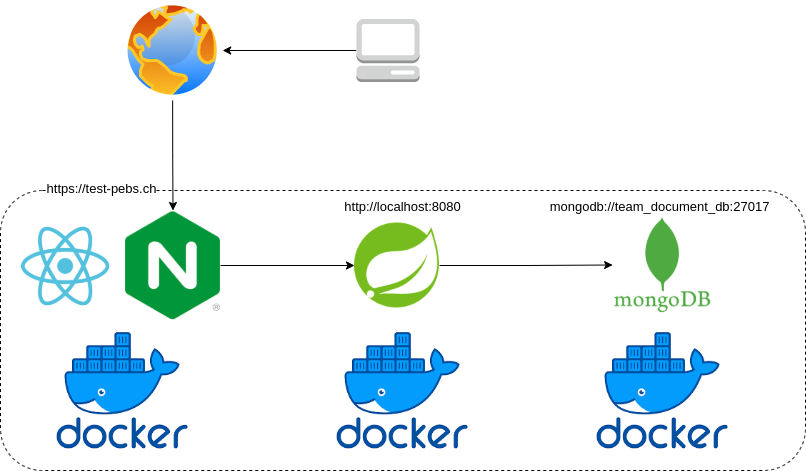
\includegraphics[width=\textwidth,keepaspectratio]{deployment-view}
    \caption{Deployment Übersicht}
    \label{fig:Deplyoment}
\end{figure}

    \section{Fazit}

Die Lösung funktioniert grundsätzlich.
Es ist möglich parallel ein Dokument auf einem öffentlich erreichbaren Server gemeinsam zu erarbeiten.
Die funktionalen Anforderungen an die Applikation sind umgesetzt.

Der Ansatz im Backend mit einem reaktiven Stack zu arbeiten und Updates über die Eventsource zu versenden funktioniert sehr gut.
Neue Funktionalität könnte elegant mit zusätzlichen Command-Types hinzugefügt und in die Processor Chain eingebunden werden.
Der Processor erreichte im isolierten Lasttest eine durchschnittliche Verarbeitungszeit von 4 ms für einen einzelnen Command.
Der Application Test von Controller bis zur Eventsource brauchte im Schnitt 40 ms für die komplette Verarbeitung.

Analog scheint auch der Ansatz im Frontend mit React und Redux gut zu funktionieren.
Die Verarbeitung der Updates von der Eventsource lässt sich mit dem gleichen Prinzip wie im Backend einfach erweitern.
Ein neuer Command entspräche dann einer neuen Funktion im Reducer.
Die Redux Komponenten kommen ohne eigene Logik aus, was die gesamte Frontendapplikation übersichtlich und einfach zu warten macht.

Was sich retrospektiv als Fehler erwiesen hat, war die Entscheidung die Commands aus dem Frontend via HTTP an den Server zu senden.
Für jedes Update wird eine TCP Verbindung aufgebaut und entsprechend auch gewartet bis diese wieder abgebaut ist.
Das führt bei schnellen aufeinanderfolgenden Updates über das Internet zu einem Request-Stau.

Treffen am Server mehr Requests ein als dieser verarbeiten kann ist auch die Reihenfolge der eingehenden Commands nicht mehr garantiert.

Diese Probleme wurden erst nach erfolgreichem Deployment auf dem öffentlichen Server sichtbar.
Aufgrund des schon fortgeschrittenen Projektstandes haben wir dieses Grundkonzept nicht gänzlich überarbeitet, sondern versucht das Netzwerk mit einer debounce funktion zu entlasten.

Die Konfliktbehandlung des Backends geht davon aus, dass Updates in der korrekten Reihenfolge (FIFO) ankommen.
Da es dennoch noch vorkommen kann, dass sich einzelne Requests überholen und die eigenen Updates vom Client direkt im Redux Store angewendet werden, können inkonsistente Zustände im Frontend entstehen.

Der vermeintliche Vorteil, dass kein Session-Management notwendig ist, wird hinfällig, sobald Informationen über andere Benutzer allen Clients zur Verfügung stehen sollen.

Aus diesen Gründen würden wir die gesamte Lösung auf Websockets umbauen bei ansonst gleichbleibender Architektur.
%%---APPENDIX----------------------------------------------------------------------------

    \listoffigures

\end{document}
